\documentclass[12pt, a4paper]{article}
\usepackage[a4paper, left=2cm, right=2cm, top=3cm, bottom=3cm]{geometry}

\usepackage[english]{babel}
\usepackage[utf8]{inputenc}
\usepackage{fancyhdr}

\usepackage{enumitem}
\usepackage{amsmath}
\usepackage{amsfonts}
\usepackage{mathtools}
\usepackage{listings}

\usepackage{array}

\usepackage{tikz}
\usetikzlibrary{arrows.meta,shapes.multipart}

\pagestyle{fancy}
\fancyhf{}
\lhead{Tutorium 02 \\ Abgabegruppe 01}
\chead{Blatt 08 \\ DatKom}
\rhead{Andrés Montoya, 405409 \\ Til Mohr, 405959}

\begin{document}

\begin{center}\fcolorbox{red}{yellow}{\begin{minipage}{35em}
	Bei uns war ursprünglich noch ein Dritter in unserer Abgabegruppe eingeteilt. Wir haben ihn vor über einer Woche versucht per E-Mail zu erreichen, leider erfolglos.\\
	Nach Ablauf der Anmeldefrist zu den Abgabegruppen haben wir gesehen, dass diese Person leider unsere Abgabegruppe verlassen hat.\\
	Bisher konnten wir noch keinen Dritten für unsere Abgabegruppe finden.\\
	Uns wurde auch seit dem letzten Blatt keine weitere Person zugeteilt.
\end{minipage}}\end{center}



\section*{Aufgabe 8.1}
\begin{enumerate}[label=\alph*)]
	\item	Mit dem ersten Paket teilt Host 1 Host 2 seine Initialparameter aus. Mit dem zweiten Paket bestätigt Host 2 diese und teilt Host 1 seine Initialparameter aus. Mit dem dritten Paket bestätigt Host 1 diese. Würde man diese Bestätigung wegfallen lassen, so könnte es Vorkommen, dass beispielsweise die Sequenznummer von Host 2 nicht mit Host 1 synchronisiert ist. Dadurch wäre die Kommunikation gestört.
	\item	Nein, wäre noch sinnvoll: Router verwerfen Pakete absichtlich bei Stau. Dann würde ja ein solches Paket nicht zuverlässig übertragen werden.
	\item	Ja. Das Paket wird als verloren anerkannt, wenn es nach RTT immer noch nicht bestätigt wurde, oder wenn nach dem verlorenen ACK noch ein weiteres / weitere ACKs eintreten, sodass das Paket wegen 3-ACKs retransmittet wird.
	\item	Eigenschaften: Schnelligkeit und Effizienz.\\
			Funktion: Ports - Man kann verschiedene Services parallel nutzen, wie bei TCP.
	\item	Ja. Man kann einen weiteren Dienst / Protokoll basierend auf UDP entwickeln, welche dann zuverlässig ist (genauso wie TCP auf IP ist).
\end{enumerate}


\newpage


\section*{Aufgabe 8.2}
\begin{enumerate}[label=\alph*)]
	\item	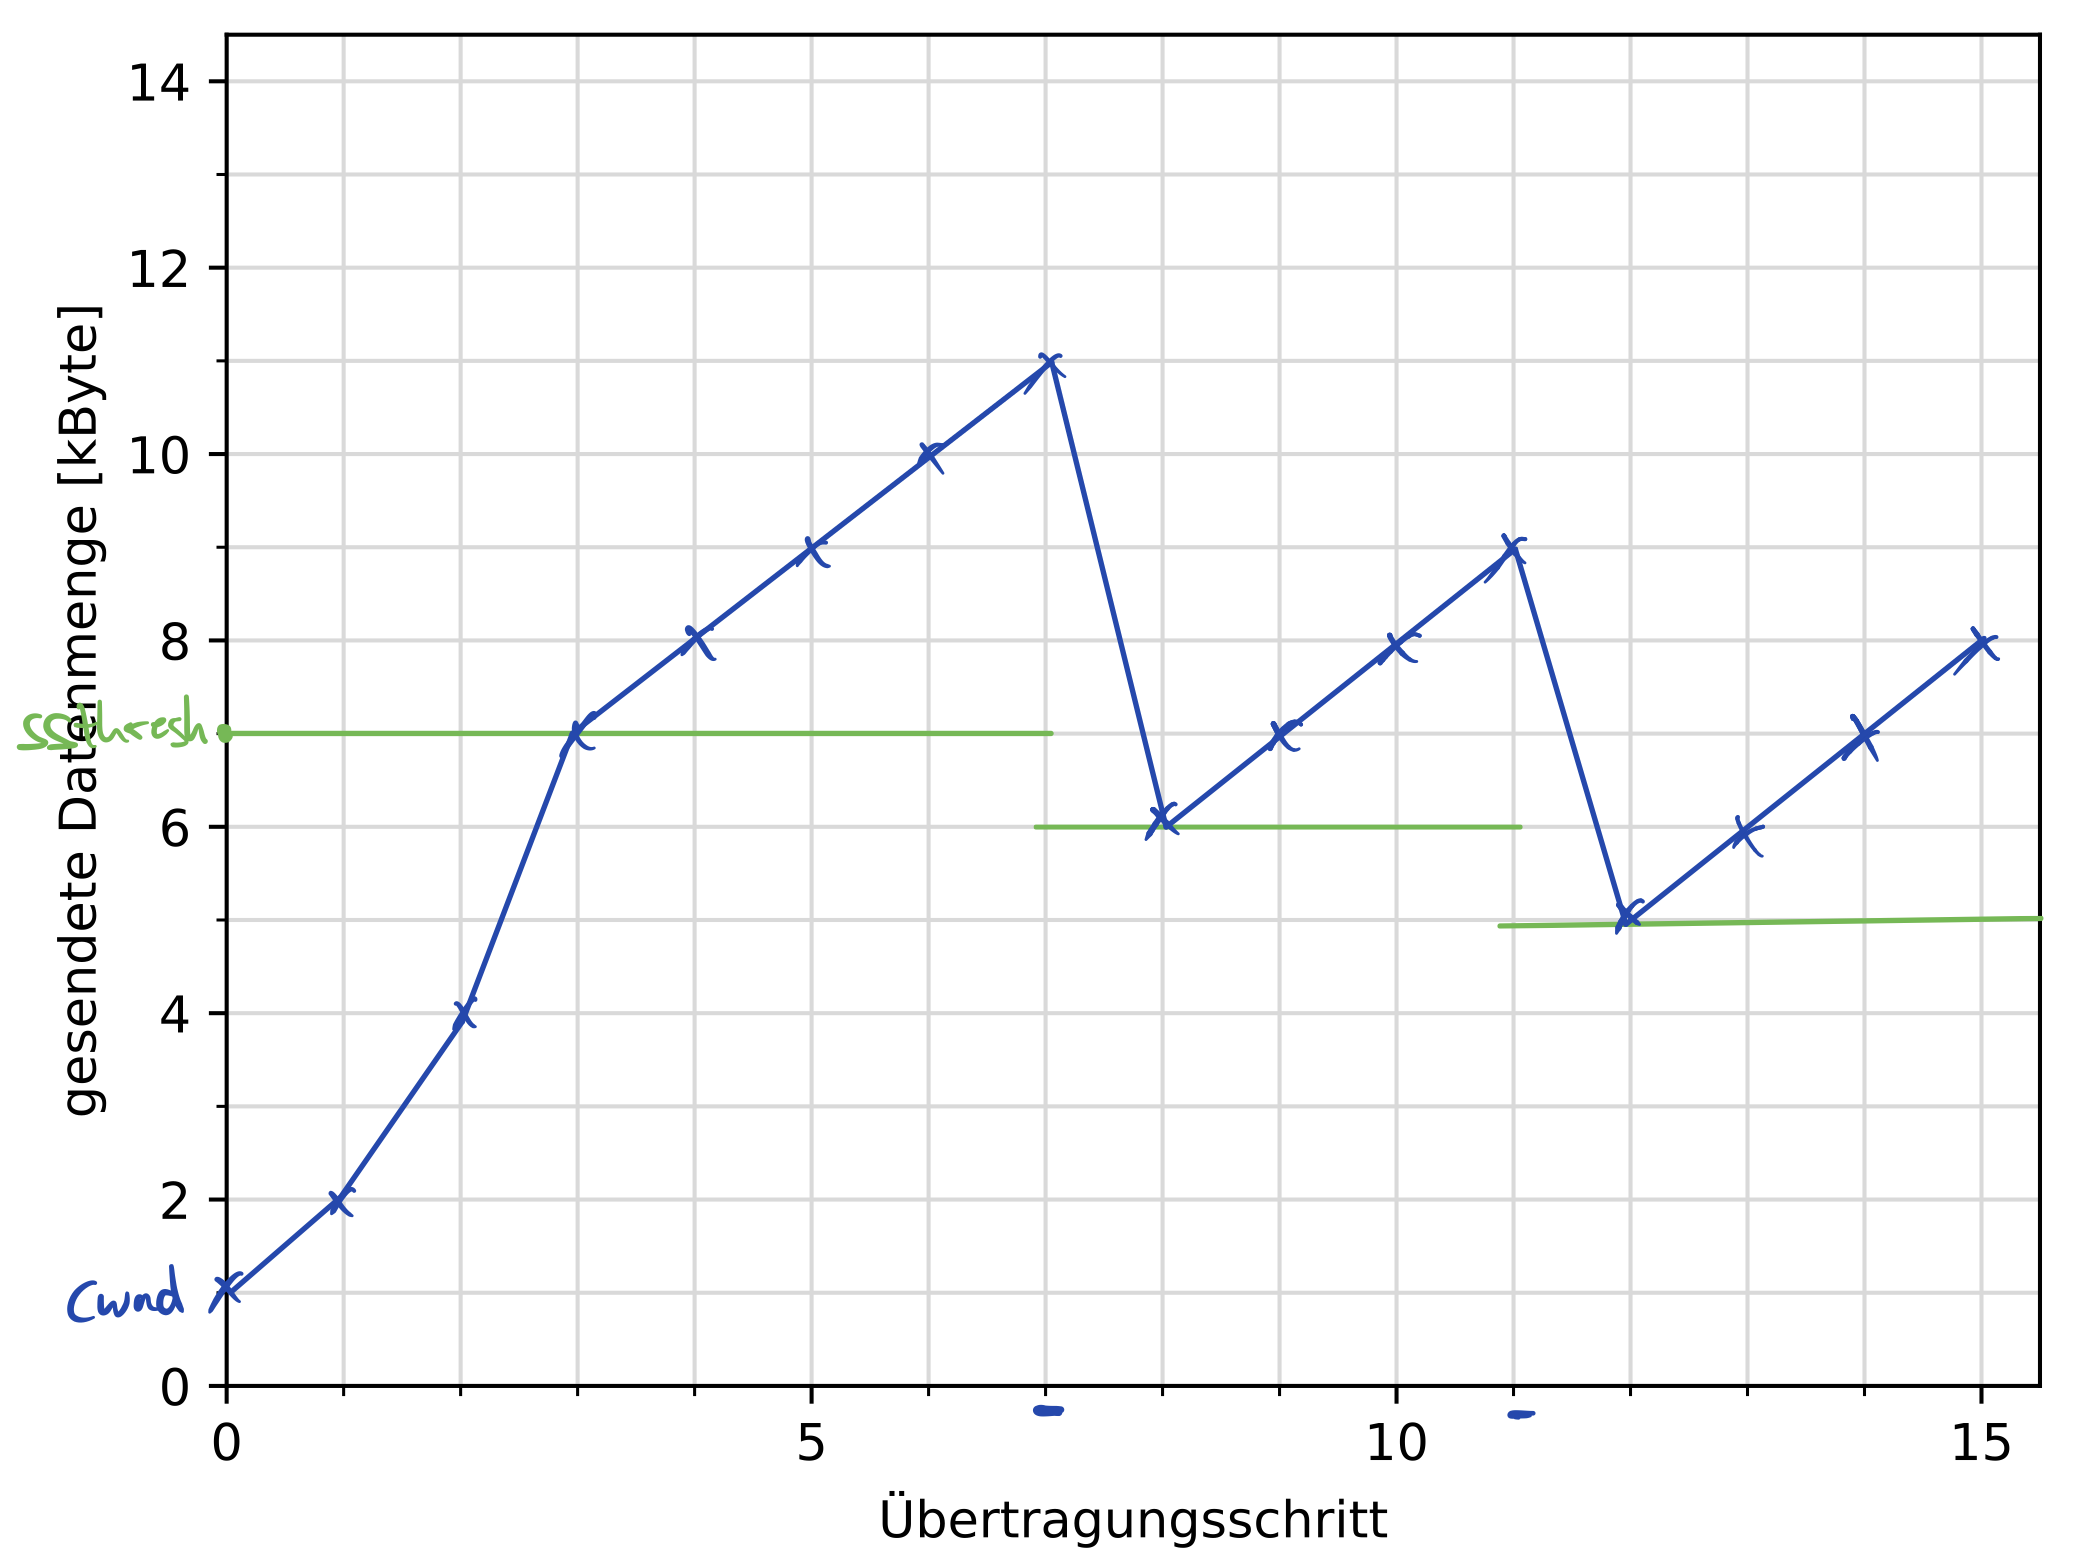
\includegraphics[scale=0.45]{8.2_a).png}
	\item	\begin{enumerate}[label=\roman*)]
				\item	Nach 4 Übertragungsschritten ist \verb|cwnd = ssthresh|. Nach 4 weiteren Schritten ist also \verb|cwnd = ssthresh + 4 kB = 12 kB|.
				\item	\verb|(1+2+4+8+9+10+11+12) kB = 57 kB|
				\item	\verb|30 kB|, da sonst würde der Empfangspuffer überlaufen und es würden Pakete verworfen werden müssen, was zu einer Erniedrigung von \verb|cwnd| führt.
			\end{enumerate}
	\item	Angenommen im Netzwerk kommunizieren noch andere Geräte und jeder Datenaustausch läuft durch einen Router. Dann kann es sein, dass andere Rechner vorher mehr kommuniziert haben, weshalb der Router aufgrund von Stau ein Paket verwerfen musste (voriges lokales Maximum). Wenn jetzt sonst niemand mehr im Netzwerk kommuniziert, können wir offensichtlich mit einer höheren \verb|cwnd| senden.
\end{enumerate}


\newpage


\section*{Aufgabe 8.3}
\begin{enumerate}[label=\alph*)]
	\item	Es gilt $\mathcal{P} = \mathcal{C} = \{A, \dots, Z\}^*$ und $\mathcal{K} = \{A, \dots, Z\}$.  Es gilt offensichtlich $\vert \mathcal{K} \vert < \vert \mathcal{P} \vert$. Nach Claude Shannon ist der Caesar-Cipher nicht perfekt.
	\item	Jetzt gilt nun dass $\vert \mathcal{K} \vert = \vert \mathcal{C} \vert = \vert \mathcal{P} \vert$. Zudem gibt es für alle $m_i$ und $c_i$ aufgrund von Modulo nur ein $\kappa_i$, sodass $c_i = m_i + \kappa_i \mod 26$. Da dies für alle $i \in \mathbb{N}$ gilt, gibt es für jedes $c \in \mathcal{C}, m \in \mathcal{P}$ genau ein $\kappa \in \mathcal{K}$, sodass $c = m + \kappa \mod 26$.\\
			Nach Shannon's Theorem ist diese Variante des Caesar Cipher perfekt.
\end{enumerate}


\newpage


\section*{Aufgabe 8.4}
\begin{enumerate}[label=\alph*)]
	\item	\begin{enumerate}[label=\roman*.]
				\item	Wiederholungen des Schlüssels äußern sich, wenn im verschlüsselten Text an unterschiedlichen Stellen dieselben Zeichenfolgen vorkommen. Dies kann indizieren, dass der Schlüssel wiederholt and derselben Stelle/Index denselben Klartext verschlüsselt hat.
				\item	Ist dies der Fall, so kann man anhand der Zeichenlänge die minimale Schlüssellänge bestimmen. Weiterhin kann man damit noch die Zeichen bis an den Start des Ciphertexts zurückzählen, und so somit die minimale Schlüssellänge womöglich genauer bestimmen:\\
						Angenommen man findet eine sich wiederholende Zeichenfolge der Länge $m$ im Ciphertext und man geht davon aus, dass der Schlüssel sich hier wiederholte. Dann beträgt die minimale Schlüssellänge $m$. Beginnt die Zeichenfolge im $i$-ten Zeichen im Ciphertext, so ist die minimale Schlüssellänge $m'$, sodass $\lfloor \frac{i}{m} \rfloor = \frac{i}{m'} \in \mathbb{N}$.
				\item	In Zeile 2 und Zeile 3 sind solche Zeichenfolgenwiederholungen. Die längere Zeichenfolge beträgt $12$ Zeichen. Der Schlüssel beträgt $16$ Zeichen (Vorgehensweise oben).
			\end{enumerate}
	\item	Key: \verb|DATKOM| - wie zu erwarten.\\
			\textit{Der Link geht nicht.}
\end{enumerate}


\end{document}